\chapter{Specific Requirements}

\section{External Interface Requirements}

\subsection{User Interfaces}

% screenshots here
\begin{figure}[h]
	\centering
	% \captionsetup{justification=centering,margin=1cm}

	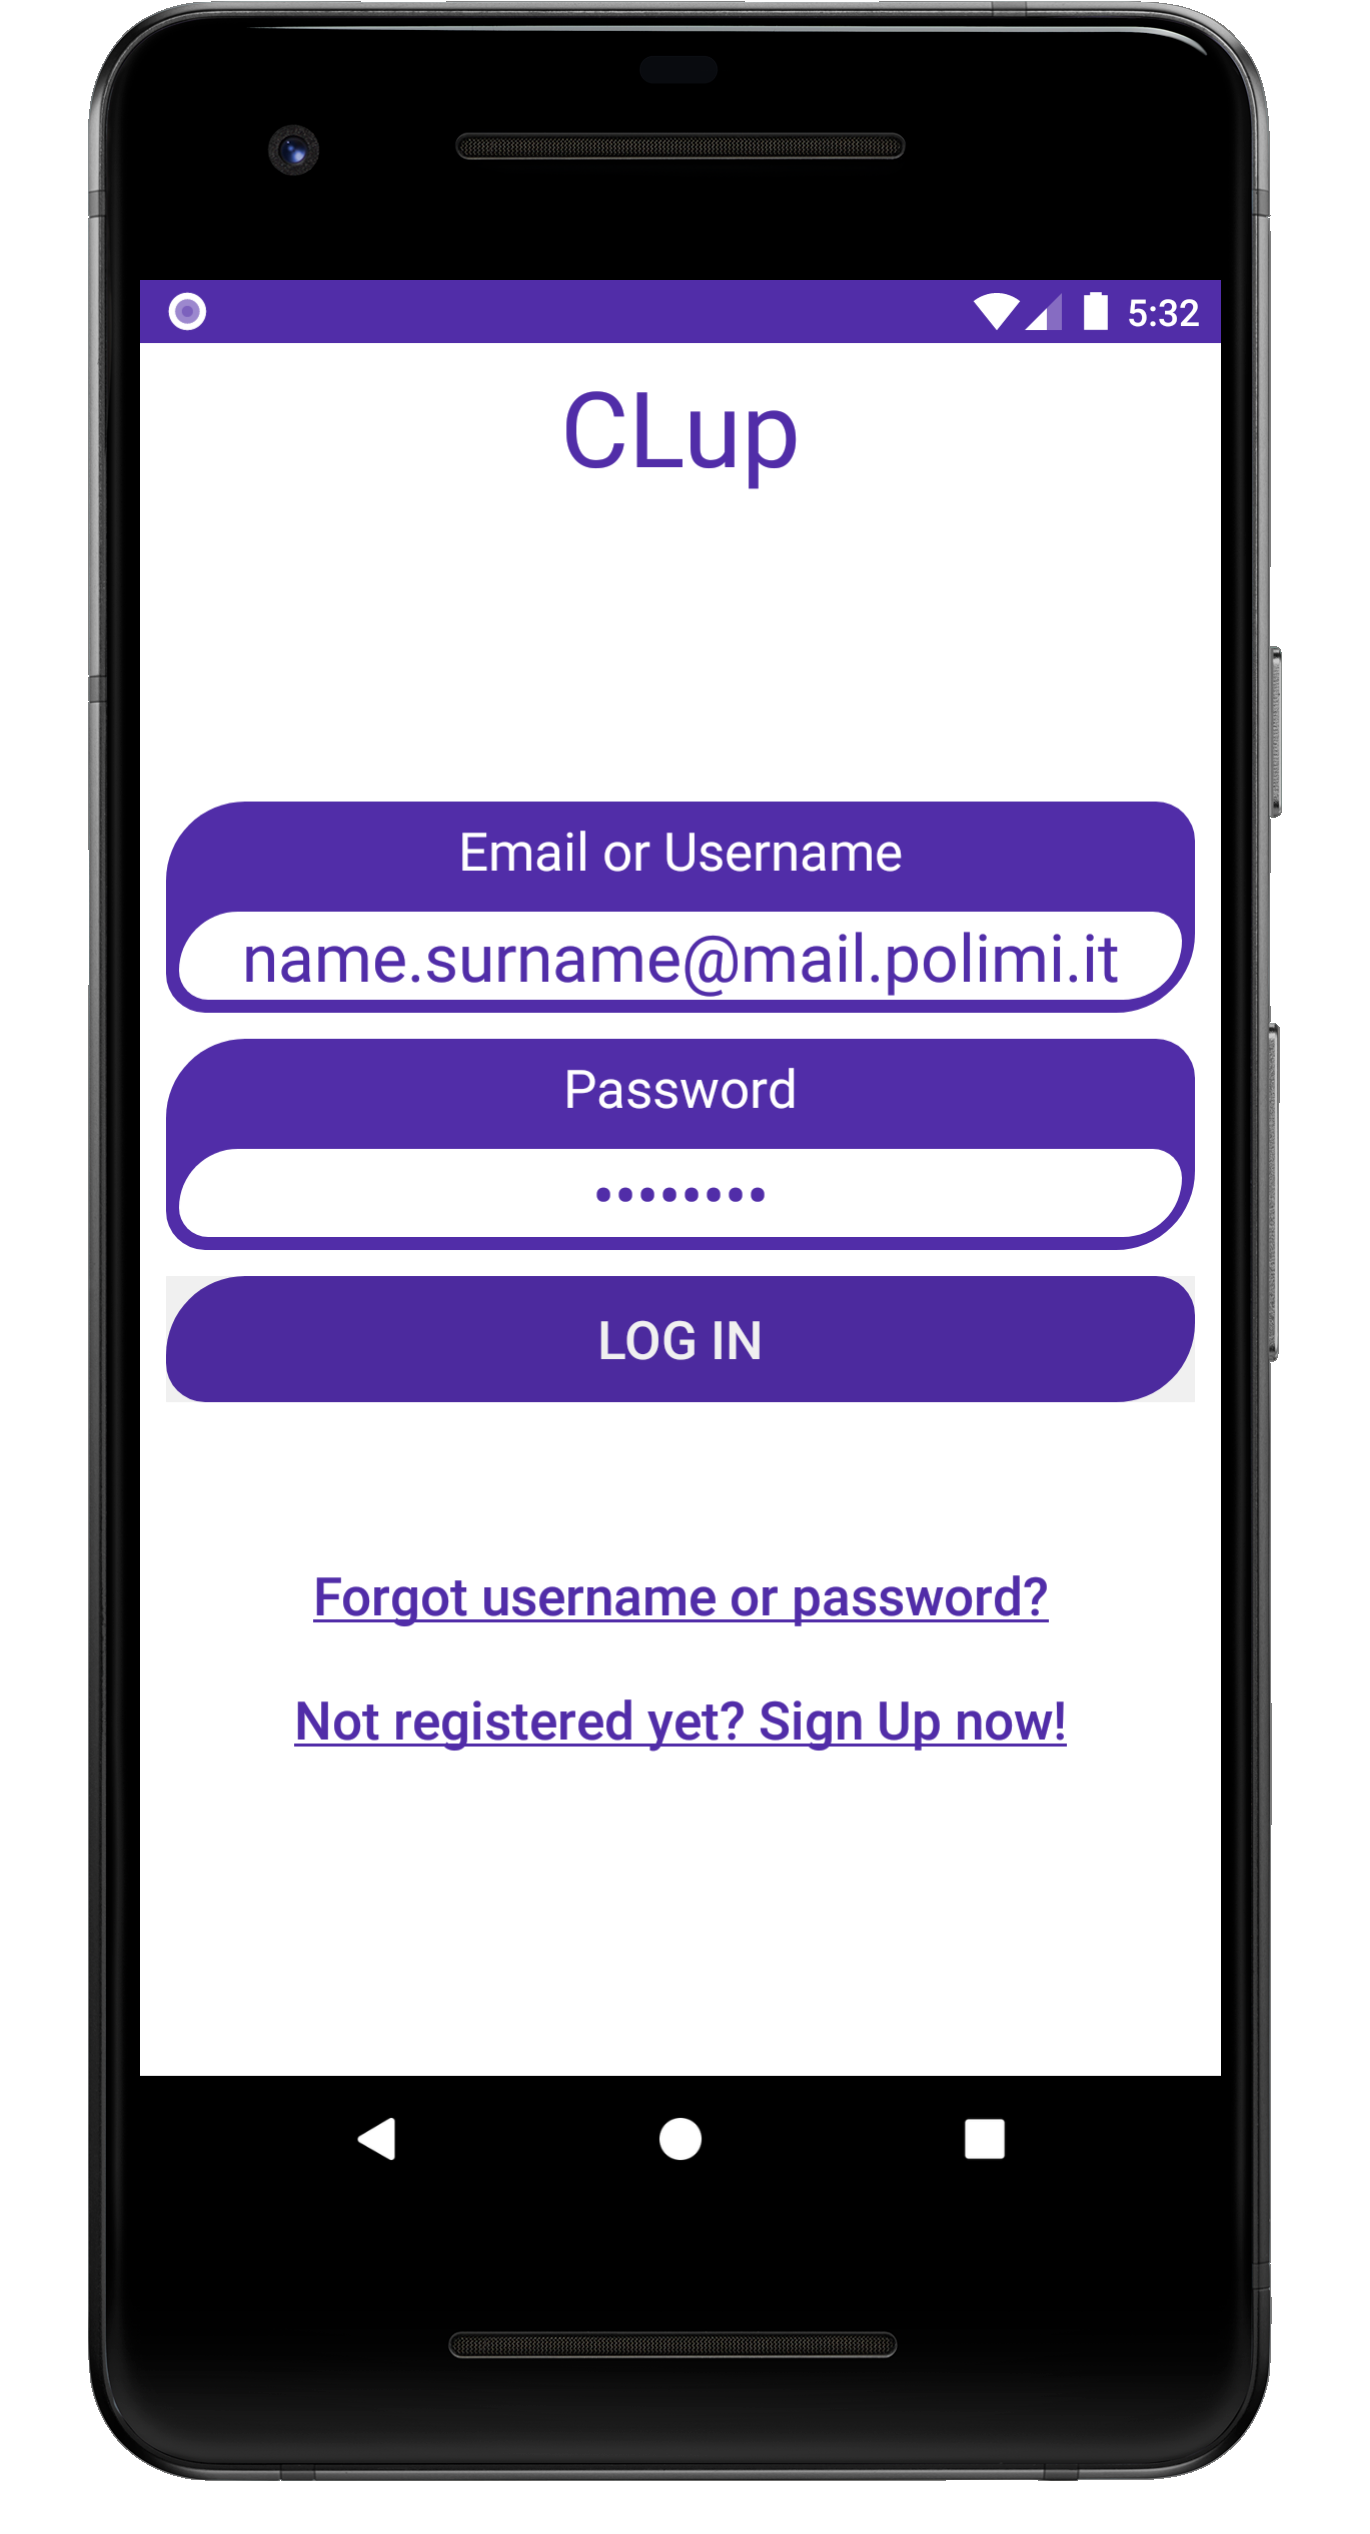
\includegraphics[width=0.5\textwidth]{images/log_in.png}
	\caption{Log In page.}
	\label{customersUseCasesDiagram}
\end{figure}

\begin{figure}[h]
	\centering
	% \captionsetup{justification=centering,margin=1cm}

	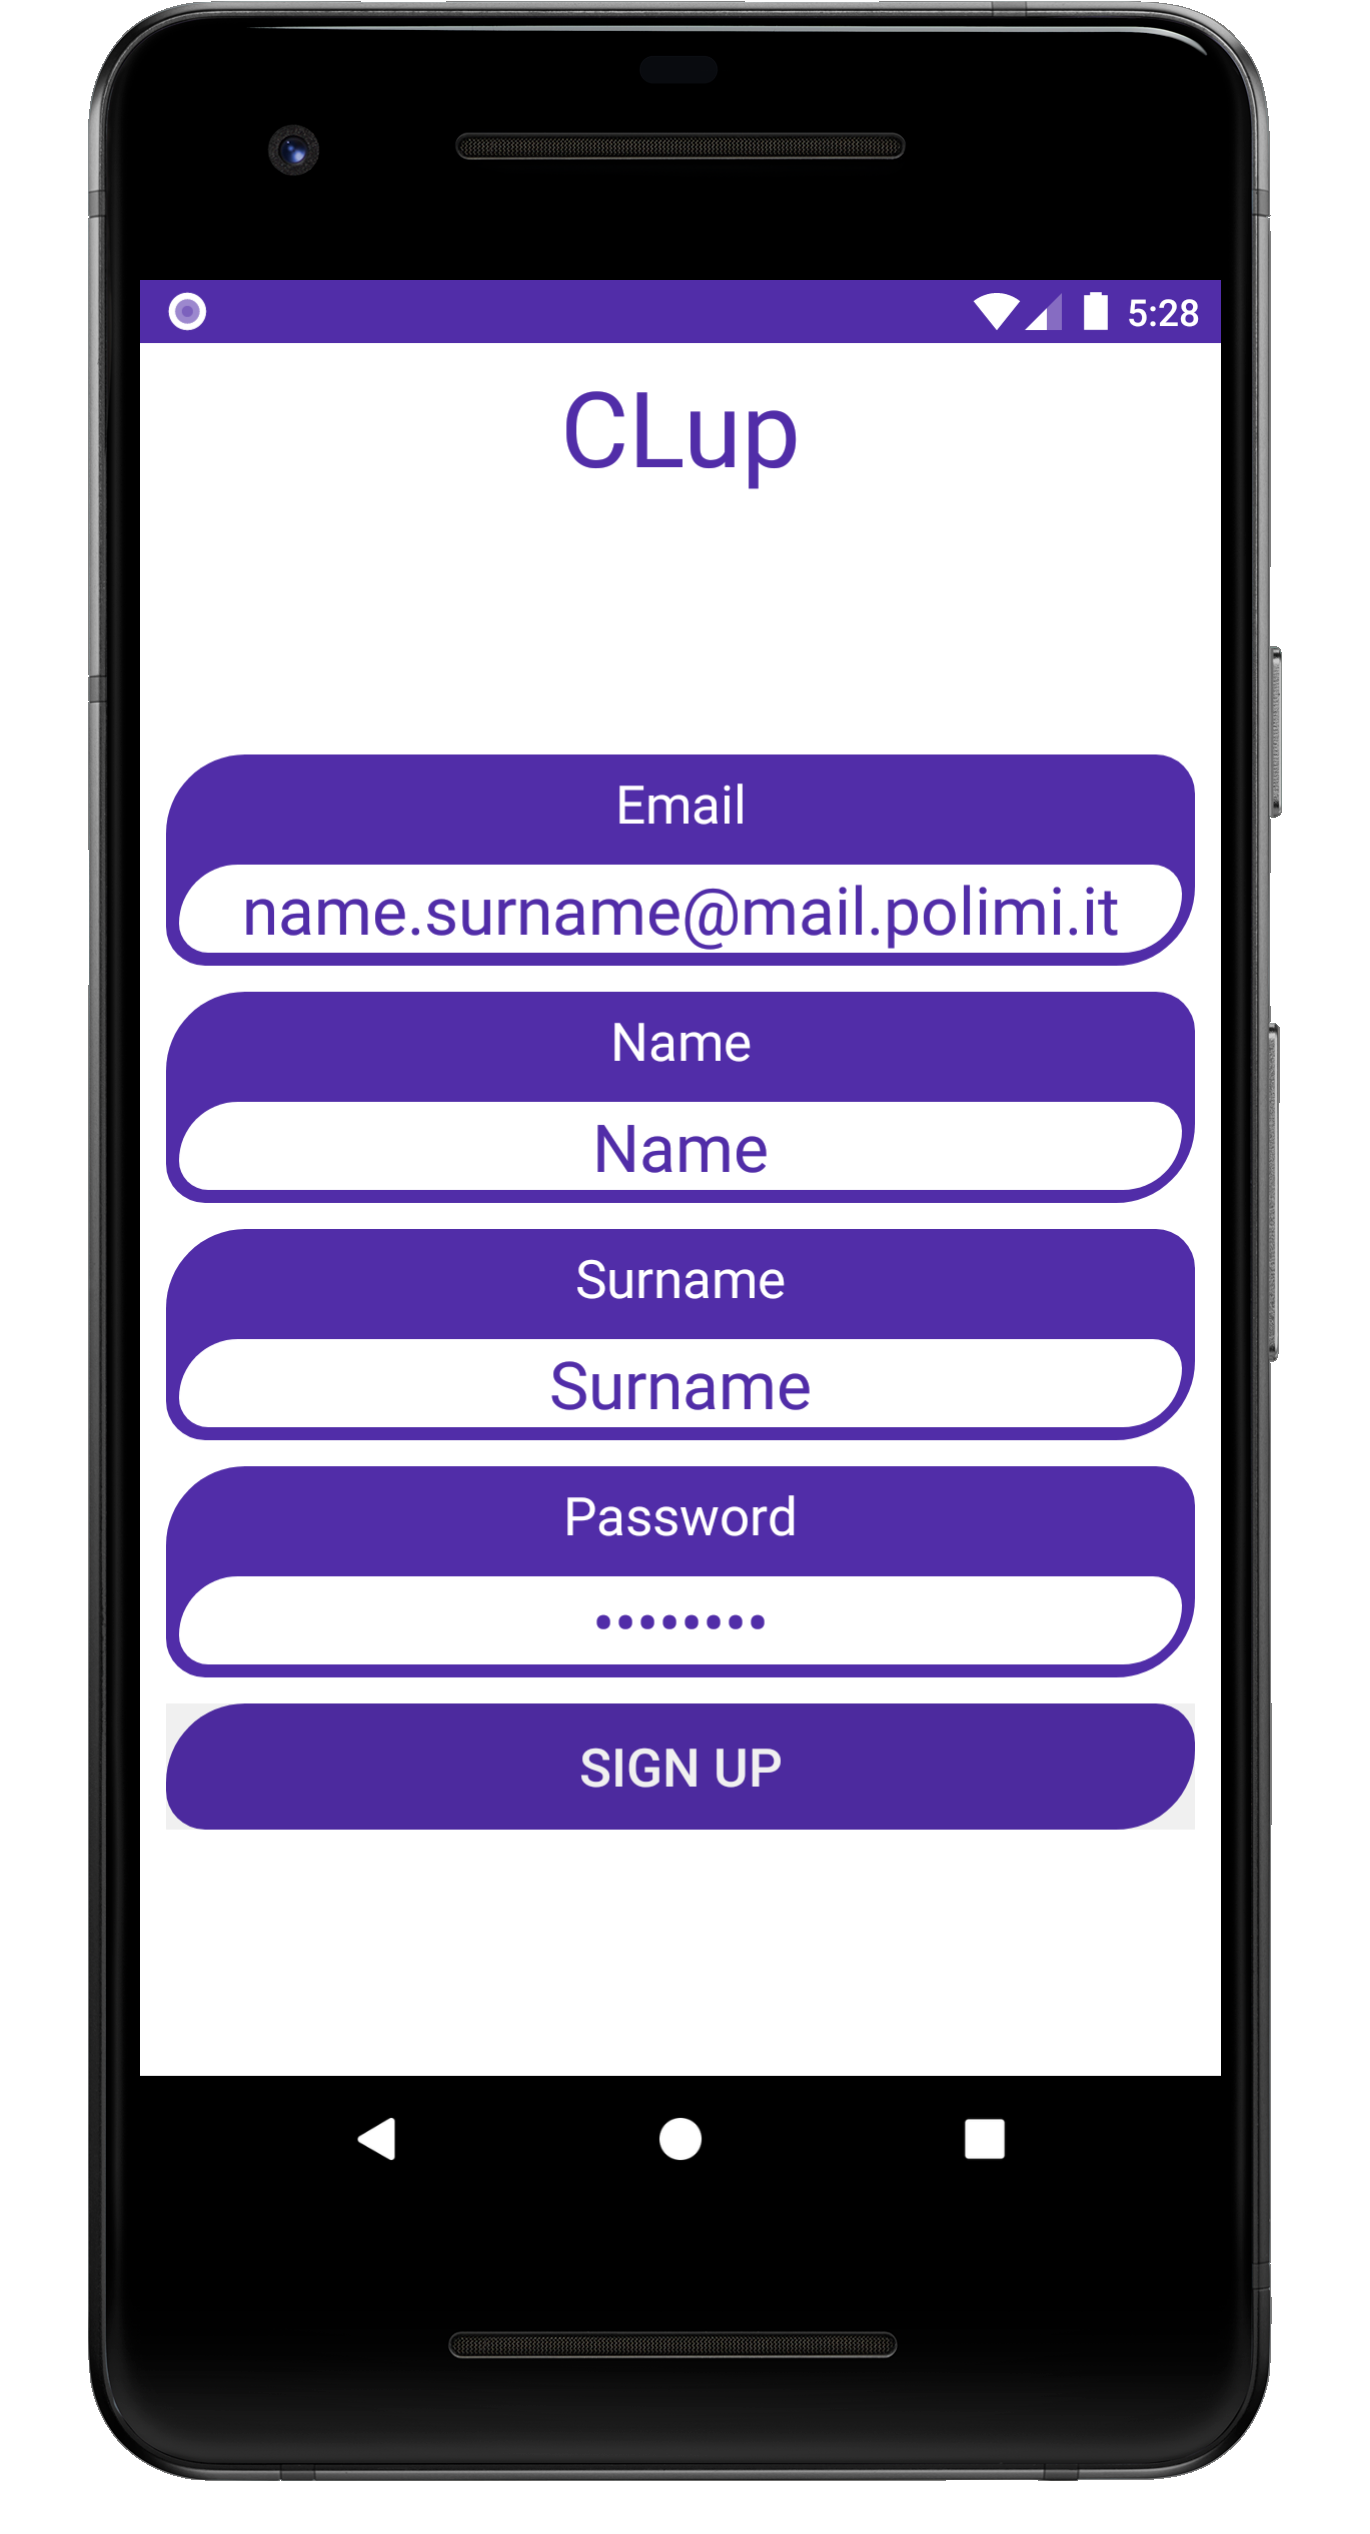
\includegraphics[width=0.5\textwidth]{images/sign_up.png}
	\caption{Sign Up page.}
	\label{customersUseCasesDiagram}
\end{figure}


\subsection{Hardware Interfaces}
\subsection{Software interfaces}
\subsection{Communications Interfaces}

\section{Functional Requirements}

\subsection{Requirements}

\subsection{Definition of Use Case Diagrams}

Bla bla bla...

\begin{figure}[h]
	\centering
	% \captionsetup{justification=centering,margin=1cm}

	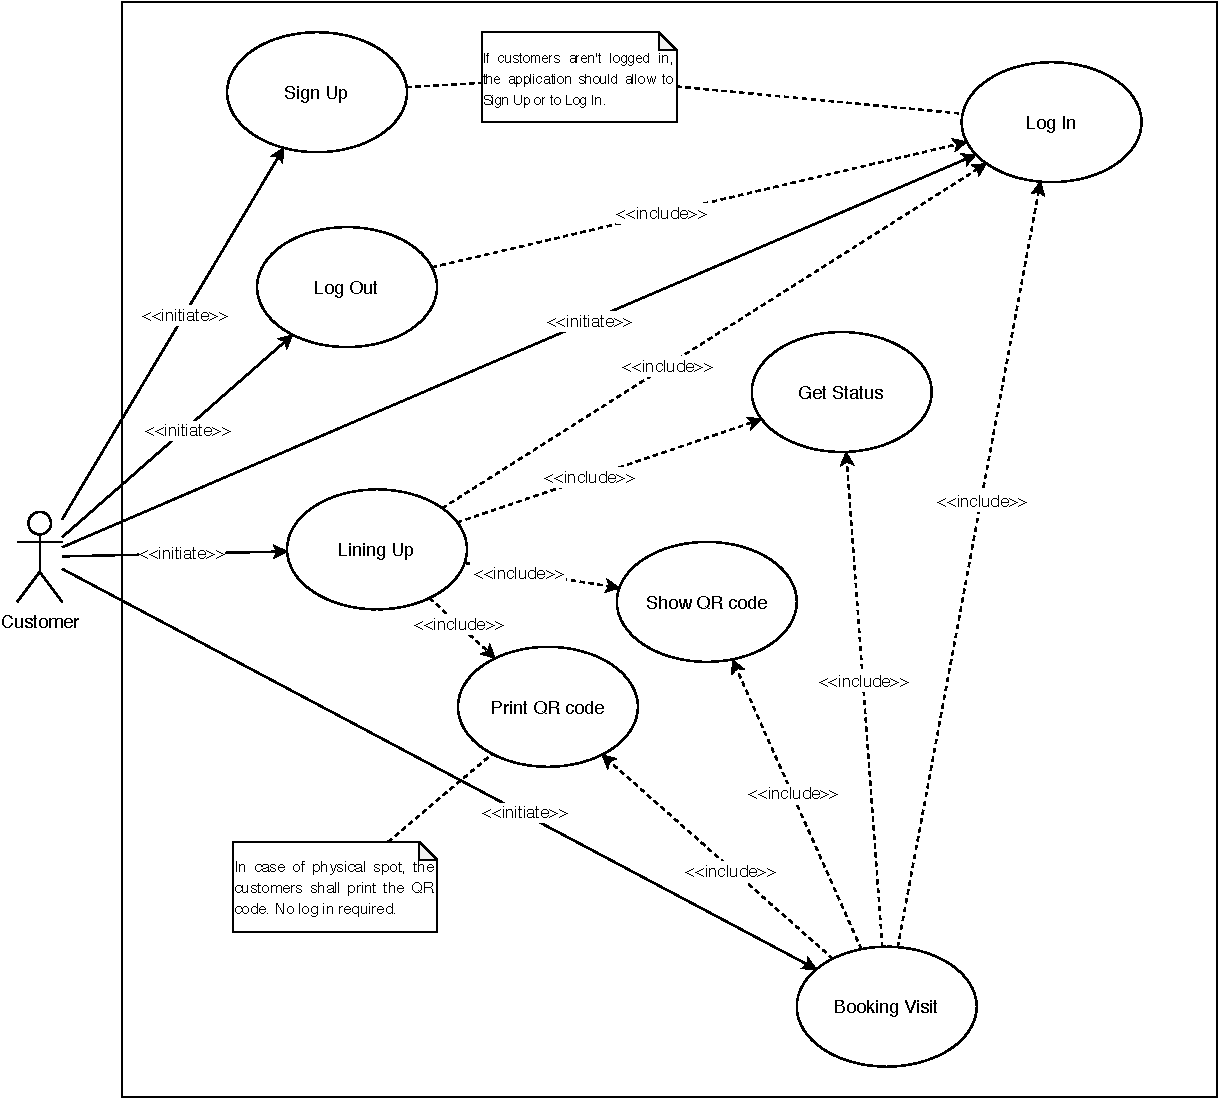
\includegraphics[width=1.0\textwidth]{images/customers_use_cases_diagram.pdf}
	\caption{Customers use cases diagram.}
	\label{customersUseCasesDiagram}
\end{figure}

\begin{table}[h!]
\centering
\begin{tabular}{| m{0.3\textwidth} | m{0.7\textwidth} |} 
	\hline
	\textbf{Name} & Sign Up \\ 
	\hline
	\textbf{Actor} & Customer \\ 
	\hline
	\textbf{Entry Conditions} & Customer is on the Sign Up page. \\ 
	\hline
	\textbf{Event Flows} &
	\begin{itemize}
		\item Customer inserts the requested information in the form.
		\item Customer clicks on the Sign Up button.
	\end{itemize} \\ 
	\hline
	\textbf{Exit Conditions} & Sign Up completed successfully and customer is logged in. \\ 
	\hline
	\textbf{Exceptions} &
	\begin{itemize}
		\item Customer's username already in use.
		\item Empty form field.
		\item Policy agreement rejected.
		\item Lost Internet connection.
	\end{itemize} \\ 
	\hline
\end{tabular}
\caption{Customer - use case: \textbf{Sign Up}.}
\label{tableSignUp}
\end{table}

\begin{table}[h!]
\centering
\begin{tabular}{| m{0.3\textwidth} | m{0.7\textwidth} |} 
	\hline
	\textbf{Name} & Log In \\ 
	\hline
	\textbf{Actor} & Customer \\ 
	\hline
	\textbf{Entry Conditions} & Customer is on the Log In page. \\ 
	\hline
	\textbf{Event Flows} &
	\begin{itemize}
	\item Customer inserts the requested information in the form.
	\item Customer clicks on the Log In button.
	\end{itemize} \\ 
	\hline
	\textbf{Exit Conditions} & Log In completed successfully and customer redirected to Home page. \\ 
	\hline
	\textbf{Exceptions} &
	\begin{itemize}
	\item Customer's username or password incorrect.
	\item Empty form field.
	\item Lost Internet connection.
	\end{itemize} \\ 
	\hline
\end{tabular}
\caption{Customer - use case: \textbf{Log In}.}
\label{tableLogIn}
\end{table}

\begin{table}[h!]
\centering
\begin{tabular}{| m{0.3\textwidth} | m{0.7\textwidth} |} 
	\hline
	\textbf{Name} & Log Out \\ 
	\hline
	\textbf{Actor} & Customer \\ 
	\hline
	\textbf{Entry Conditions} & Customer is on the Log Out page. \\ 
	\hline
	\textbf{Event Flows} &
	\begin{itemize}
	\item Customer clicks on the Log Out button.
	\end{itemize} \\ 
	\hline
	\textbf{Exit Conditions} & Log Out completed successfully and customer redirected to the Sign Up/Log In page. \\ 
	\hline
	\textbf{Exceptions} &
	\begin{itemize}
	\item Customer already logged out.
	\item Lost Internet connection.
	\end{itemize} \\ 
	\hline
\end{tabular}
\caption{Customer - use case: \textbf{Log Out}.}
\label{tableLogIn}
\end{table}

\begin{table}[h!]
\centering
\begin{tabular}{| m{0.3\textwidth} | m{0.7\textwidth} |} 
	\hline
	\textbf{Name} & Lining Up \\ 
	\hline
	\textbf{Actor} & Customer \\ 
	\hline
	\textbf{Entry Conditions} & Customer is on the Home page \\ 
	\hline
	\textbf{Event Flows} &
	\begin{itemize}
	\item Customer clicks on the Lining Up button.
	\end{itemize} \\ 
	\hline
	\textbf{Exit Conditions} & Lining Up completed successfully, the application returns, to the customer, the Status page and saves the QR code in the main memory. \\ 
	\hline
	\textbf{Exceptions} &
	\begin{itemize}
	\item Previous Lining Up action was not expired.
	\item Previous Booking Visit action was not expired.
	\item Customer wasn't logged.
	\item QR code cannot be saved correctly on the main memory.
	\item Lost Internet connection.
	\end{itemize} \\ 
	\hline
\end{tabular}
\caption{Customer - use case: \textbf{Lining Up}.}
\label{tableLogIn}
\end{table}

\begin{table}[h!]
\centering
\begin{tabular}{| m{0.3\textwidth} | m{0.7\textwidth} |} 
	\hline
	\textbf{Name} & Booking Visit \\ 
	\hline
	\textbf{Actor} & Customer \\ 
	\hline
	\textbf{Entry Conditions} & Customer is on the Home page \\ 
	\hline
	\textbf{Event Flows} &
	\begin{itemize}
	\item Customer clicks on the Booking Visit button.
	\item Customer fills the form with the requested data.
	\item Customer clicks on the Submit button.
	\end{itemize} \\ 
	\hline
	\textbf{Exit Conditions} & Booking Visit completed successfully and the application returns, to the customer, the Status page. \\ 
	\hline
	\textbf{Exceptions} &
	\begin{itemize}
	\item Previous Lining Up action was not expired.
	\item Previous Booking Visit action was not expired.
	\item Customer wasn't logged.
	\item QR code cannot be saved correctly on the main memory.
	\item Lost Internet connection.
	\end{itemize} \\ 
	\hline
\end{tabular}
\caption{Customer - use case: \textbf{Booking Visit}.}
\label{tableLogIn}
\end{table}

\begin{table}[h!]
\centering
\begin{tabular}{| m{0.3\textwidth} | m{0.7\textwidth} |} 
	\hline
	\textbf{Name} & Show QR code \\ 
	\hline
	\textbf{Actor} & Customer \\ 
	\hline
	\textbf{Entry Conditions} & Customer is on the Home page \\ 
	\hline
	\textbf{Event Flows} &
	\begin{itemize}
	\item Customer clicks on the Show QR code button.
	\end{itemize} \\ 
	\hline
	\textbf{Exit Conditions} & The application shows the QR code associated to the last Lining Up, or Booking Visit, operation. \\ 
	\hline
	\textbf{Exceptions} &
	\begin{itemize}
	\item QR code hasn't be saved on the application correctly.
	\item No Lining Up, or Booking Visit, action performed. % redirect to Lining Up page ot hide button if QR code doesn't exist.
	\item Customer wasn't logged.
	\end{itemize} \\ 
	\hline
\end{tabular}
\caption{Customer - use case: \textbf{Show QR code}.}
\label{tableLogIn}
\end{table}

\begin{table}[h!]
\centering
\begin{tabular}{| m{0.3\textwidth} | m{0.7\textwidth} |} 
	\hline
	\textbf{Name} & Get Status \\ 
	\hline
	\textbf{Actor} & Customer \\ 
	\hline
	\textbf{Entry Conditions} & Customer is on the Home page. \\ 
	\hline
	\textbf{Event Flows} &
	\begin{itemize}
	\item Customer clicks on the Get Status button.
	\end{itemize} \\ 
	\hline
	\textbf{Exit Conditions} & The application returns the Get Status page showing information about the last Lining Up, or Booking Visit, operation. \\ 
	\hline
	\textbf{Exceptions} &
	\begin{itemize}
	\item No operation previously performed, therefore there is no data to show.
	\item Customer wasn't logged.
	\item Lost Internet connection.
	\end{itemize} \\ 
	\hline
\end{tabular}
\caption{Customer - use case: \textbf{Get Status}.}
\label{tableLogIn}
\end{table}

\begin{table}[h!]
\centering
\begin{tabular}{| m{0.3\textwidth} | m{0.7\textwidth} |} 
	\hline
	\textbf{Name} & Print QR code \\ 
	\hline
	\textbf{Actor} & Customer \\ 
	\hline
	\textbf{Entry Conditions} & Customer is acting on the physical spot and he is on the Print QR code page. \\ 
	\hline
	\textbf{Event Flows} &
	\begin{itemize}
	\item Customer clicks on the Print QR code button.
	\end{itemize} \\ 
	\hline
	\textbf{Exit Conditions} & The spot prints the ticket with the QR code. \\ 
	\hline
	\textbf{Exceptions} &
	\begin{itemize}
	\item Spot finished the paper.
	\item Spot finished the ink.
	\item No more empty slots for the Lining Up in the current day.
	\end{itemize} \\ 
	\hline
\end{tabular}
\caption{Customer - use case: \textbf{Print QR code}.}
\label{tableLogIn}
\end{table}


\subsection{Use Cases and Sequence/Activity Diagrams}
\subsection{Mapping on Requirements}

\section{Performance Requirements}

\section{Design Constraints}

\subsection{Standard Compliance}
\subsection{Hardware limitations}
\subsection{Any Other Constraint}

\section{Software System Attributes}

\subsection{Reliability}
\subsection{Availability}
\subsection{Security}
\subsection{Maintainability}
\subsection{Portability}